\documentclass[12pt]{beamer}

\usetheme{metropolis}
\usepackage{appendixnumberbeamer}

% Notes for pdfpc
\usepackage{pdfpc}

\usepackage{booktabs}
\usepackage[scale=2]{ccicons}

\usepackage{pgfplots}
\usepgfplotslibrary{dateplot}

\usepackage{xspace}
\newcommand{\themename}{\textbf{\textsc{metropolis}}\xspace}

%%% Frameheader with Image
\makeatletter
\setbeamertemplate{frametitle}{%
    \nointerlineskip%
    \begin{beamercolorbox}[%
        wd=\paperwidth,%
        sep=0pt,%
        leftskip=\metropolis@frametitle@padding,%
        rightskip=\metropolis@frametitle@padding,%
    ]{frametitle}%
    \metropolis@frametitlestrut@start%
    \insertframetitle%
    \nolinebreak%
    \metropolis@frametitlestrut@end%
    \hfill
    \raisebox{-1.2ex}{
        
\includegraphics[height=4ex,keepaspectratio]{images/logos/losfuzzys_logo.png}
    }
  \end{beamercolorbox}%
}
\makeatother

%%% Titlepage with LOGO
\titlegraphic{%
  \hfill
  
\includegraphics[width=6cm,height=1.6cm,keepaspectratio]{images/logos/losfuzzys_logo.png}
  \hfill

}

\title{Introduction to CTFs}
\subtitle{What are CTFs and how to get started}
\date{\today}
\author{LosFuzzys}
% \institute{TU}
% \titlegraphic{\hfill\includegraphics[height=1.5cm]{logo.pdf}}

\begin{document}

\maketitle

% \begin{frame}{Table of contents}
%   \setbeamertemplate{section in toc}[sections numbered]
%   \tableofcontents[hideallsubsections]
% \end{frame}

\section{Introduction}

\begin{frame}{\$whoarewe}
    \hspace*{-1cm}
    \begin{tabular}{cl}
        \begin{tabular}{l}
            \parbox{0.6\linewidth}{
                \begin{itemize}
                    \item $\sim$ 15 active Member
                    \item Meet every Wednesday 18:15 (Infeldgasse 16a, ground floor)
                    \item Regular compeeting in security copmetitions, host CTFs, trainings and workshops
                \end{itemize}
                \begin{figure}
                    
\includegraphics[trim=1cm 1cm 1cm 1cm,clip=true,width=0.5\linewidth]{images/qrcode.png}
                \end{figure}
            }
        \end{tabular}  &
        \begin{tabular}{c}
            \begin{figure}
                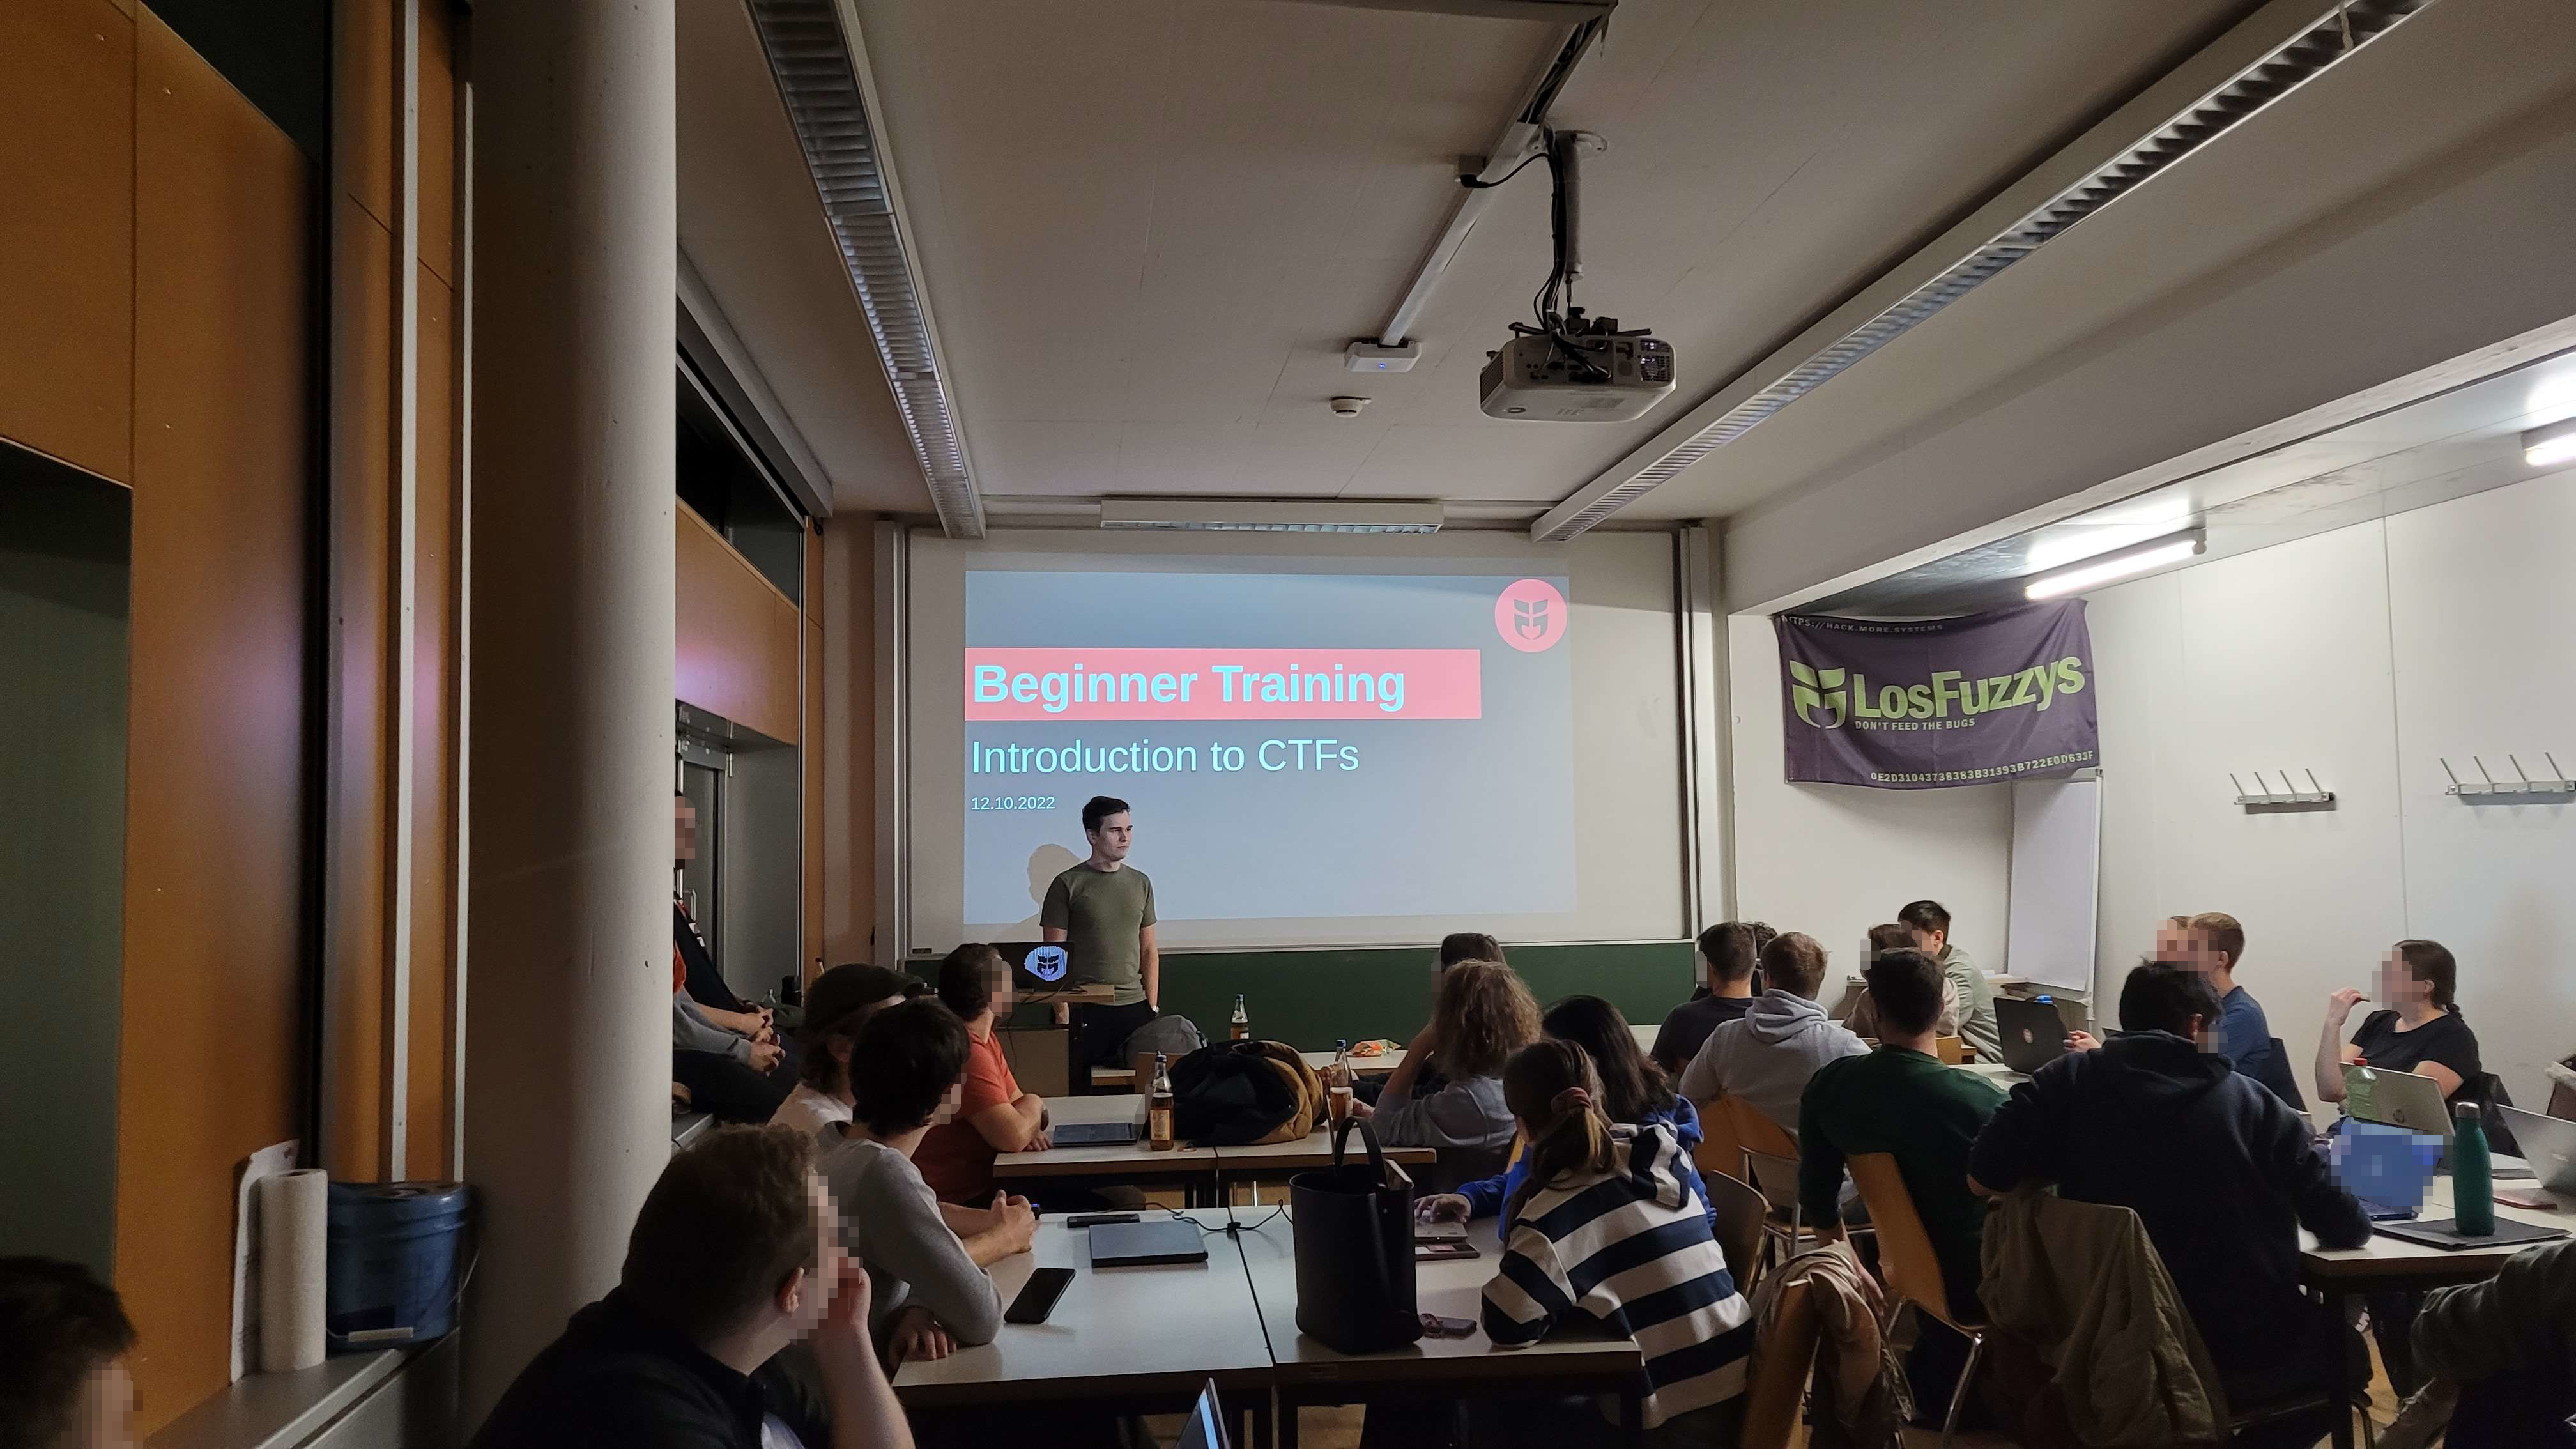
\includegraphics[width=0.45\linewidth]{images/events/Beginnertrainings2022.jpg}
            \end{figure} \\
            \begin{figure}
                \includegraphics[width=0.45\linewidth]{images/events/kdctf.JPG}
            \end{figure}
        \end{tabular}
    \end{tabular}
    \pdfpcnote{Small group of people that reguarly compeet in CTFs. Events and trainings: fuzzy.land, KaindorfCTF, Beginnertrainings 2022}
\end{frame}

\begin{frame}{Overview}
    What are CTFs?
    \begin{itemize}
        \item {\bf C}apture {\bf t}he {\bf F}lag
        \item Competitions with a focuse on cyber security
        \item Either online (mostly) of offline (typically for finals)
        \item Usually take 24 hours, 36h or even longer
    \end{itemize}
    There are usually the following gamemodes
    \begin{itemize}
        \item Jeopardy (most common)
        \item Attack-Defense
    \end{itemize}
\end{frame}

\begin{frame}{Flag?}
    \huge{LosCTF\{this\_could\_be\_a\_flag\}}
    \pdfpcnote{Praefix typically gives a hint about the CTF, curly braces, flagbody}
\end{frame}


\section{CTFTime}
\begin{frame}{ctftime.org}
    \centering
    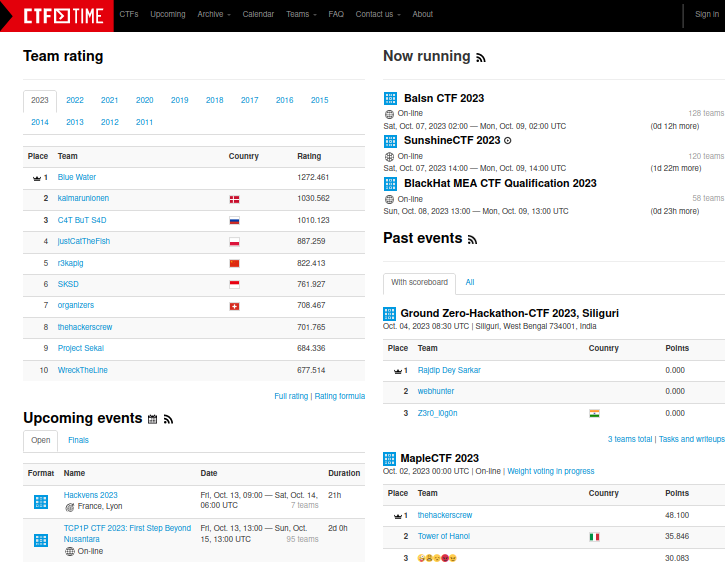
\includegraphics[width=0.8\columnwidth]{images/CTFTimeStartpage.png}
    \pdfpcnote{Overview of currently and upcomming competition, global ranking,}
\end{frame}


\section{Jeopardy-CTFs}
\begin{frame}{Challenge Categories}
    Most of the time, challenges fall in one of these Categories
    \begin{itemize}
        \item Reverse engineering
        \item Binary exploitation
        \item Websecurity
        \item Cryprography
        \item Miscellaneous
    \end{itemize}

    Other categories can be
    \begin{itemize}
        \item Web3 (Smart contract security)
        \item Digital forensics 
        \item Programming challenges
        \item Open-source intelligence gathering (OSINT)
    \end{itemize}
\end{frame}

\begin{frame}{How do Jeopardy-CTFs work?}

    \only<1>{
        \centering
        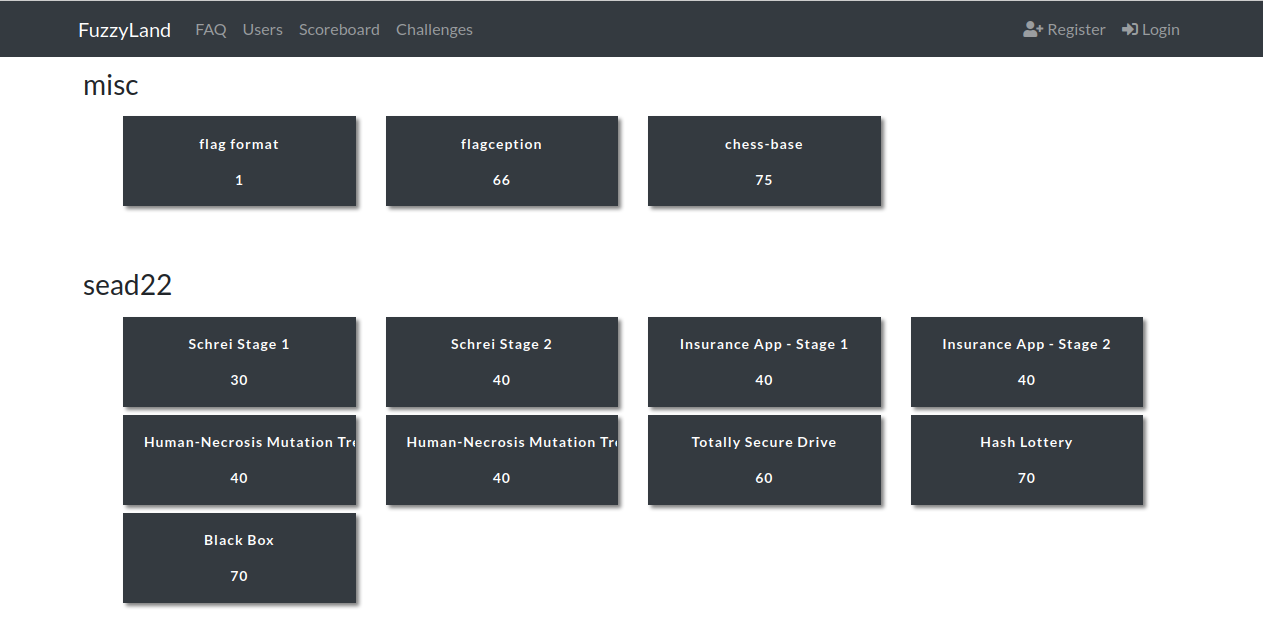
\includegraphics[width=0.95\columnwidth]{images/jeopardy_ctfs/fuzzy_land_1.png}
        \pdfpcnote{Different challenges grouped in categories; Grey = unsolved, green = solved}
    }%
    \only<2>{
        \centering
        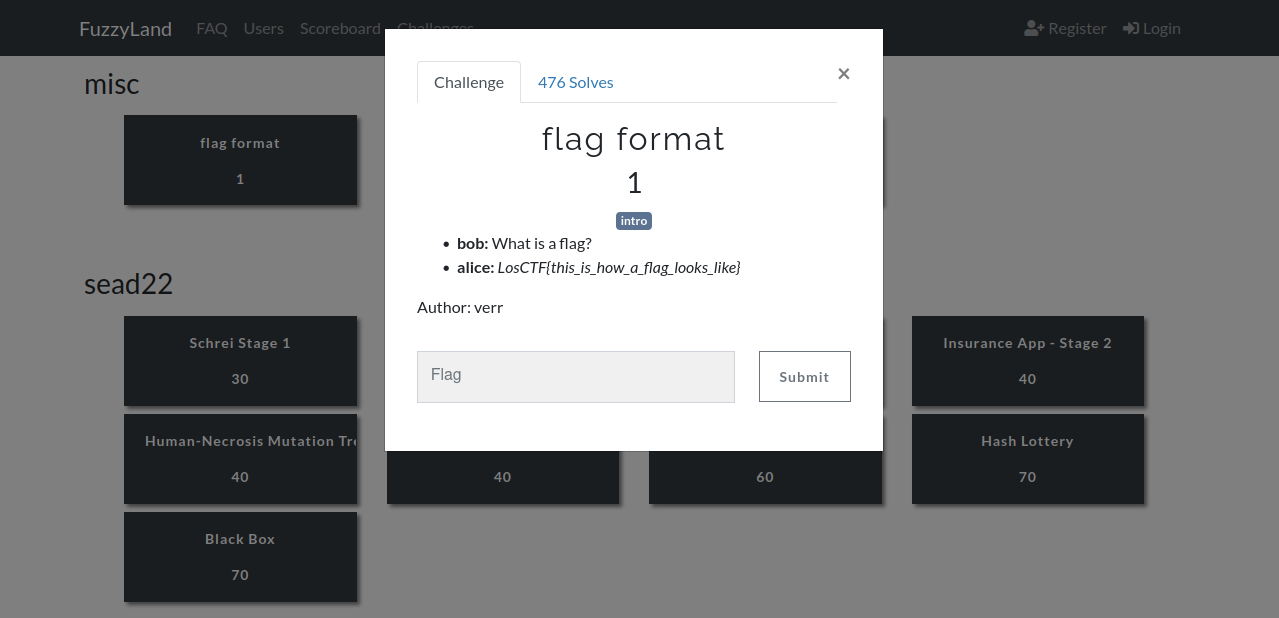
\includegraphics[width=0.95\columnwidth]{images/jeopardy_ctfs/fuzzy_land_2.png}
        \pdfpcnote{Every Challenge has a name, points, number of solves and a description}
    }%
    \only<3>{
        \centering
        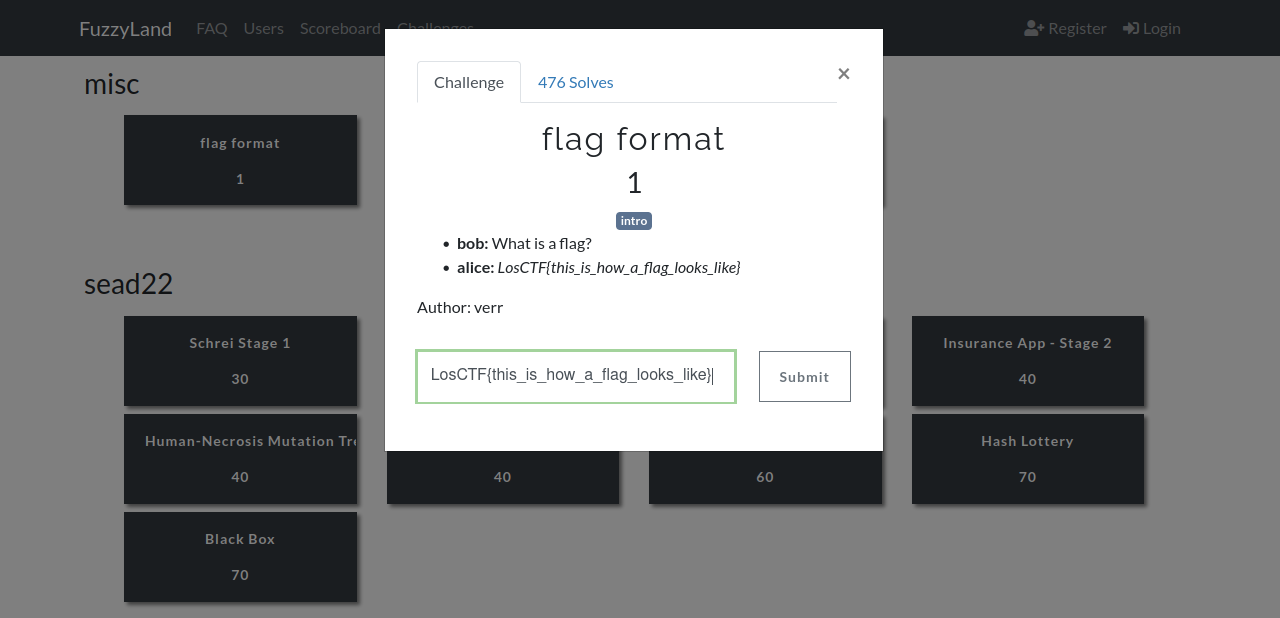
\includegraphics[width=0.95\columnwidth]{images/jeopardy_ctfs/fuzzy_land_3.png}
    }%
    \only<4>{
        \centering
        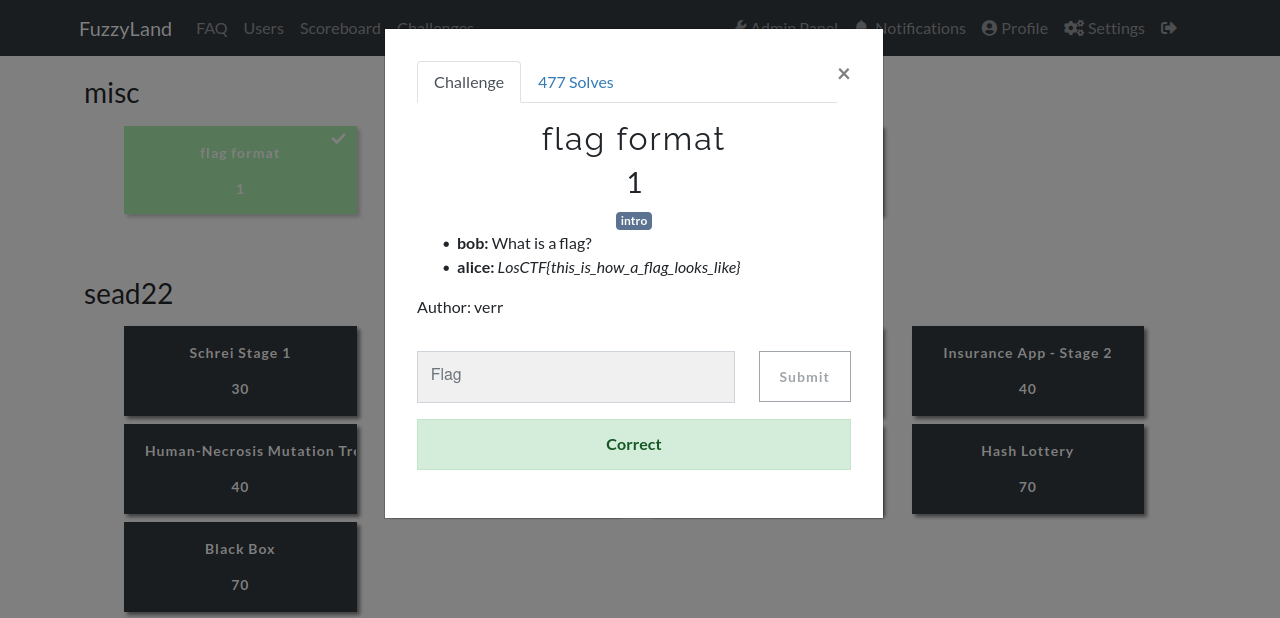
\includegraphics[width=0.95\columnwidth]{images/jeopardy_ctfs/fuzzy_land_4.png}
        \pdfpcnote{Submitting a valid flag markes the challenge as solved}
    }%

\end{frame}


\section{AD-CTFs}
\begin{frame}{Challenge Categories}
    Every team gets a server with vulnerable services \\
    Goals
    \begin{itemize}
        \item Fix the own services
        \item Exploit the other teams
    \end{itemize}

    Typical categories
    \begin{itemize}
        \item Reverse engineering
        \item Binary exploitation
        \item Websecurity
    \end{itemize}
    \pdfpcnote{Find the vulnerabilities in the own service, patch them and write exploits. Analyse network traffic in order to possiblie steam exploits from other teams}
\end{frame}

\begin{frame}{How do AD-CTFs work?}

    \only<1>{
        \centering
        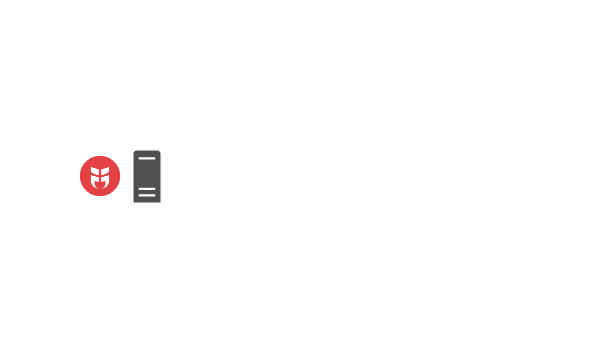
\includegraphics[width=0.95\columnwidth]{images/ad_ctfs/ad_overview_1.png}
        \pdfpcnote{Teams get a serverimage with servies; sometimes the vulnbox is alrady provided by the organizers}
    }%
    \only<2>{
        \centering
        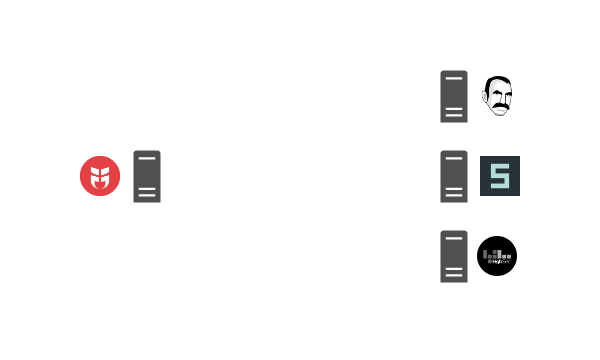
\includegraphics[width=0.95\columnwidth]{images/ad_ctfs/ad_overview_2.png}
        \pdfpcnote{Every team should have this set up (if the vulnbox is not provided); 4 different teams competing in this case}
    }%
    \only<3>{
        \centering
        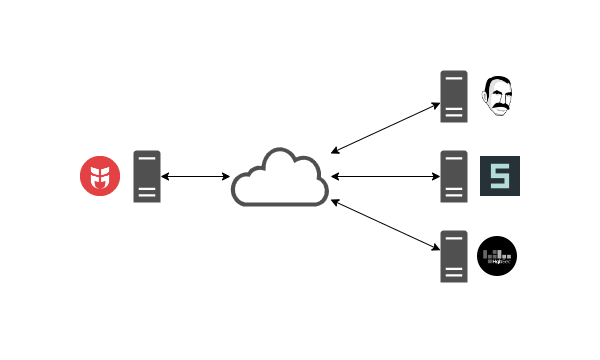
\includegraphics[width=0.95\columnwidth]{images/ad_ctfs/ad_overview_3.png}
        \pdfpcnote{Once the ctf startes, the teams connect to ga gamenetwork; typically there is a 1 houre grace periode where teams can connect to the network but can not reach each other}
    }%
    \only<4>{
        \centering
        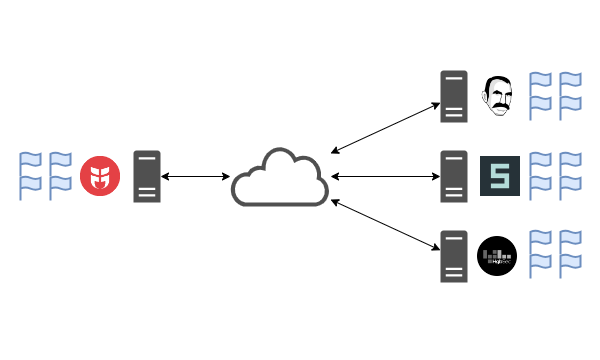
\includegraphics[width=0.95\columnwidth]{images/ad_ctfs/ad_overview_4.png}
        \pdfpcnote{Once the ctf starts, a gameserver distributes flags that are different for each team and every service.}
    }%
    \only<5>{
        \centering
        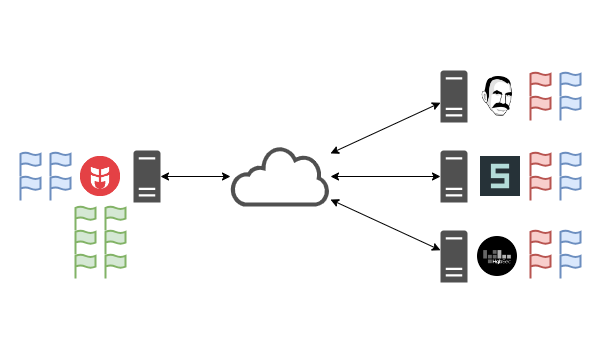
\includegraphics[width=0.95\columnwidth]{images/ad_ctfs/ad_overview_5.png}
        \pdfpcnote{In this case losfuzzys was able to attack two out of four services and gather the flags from every team}
    }%

\end{frame}


\section{Introduction Challenges}
\begin{frame}{fuzzy.land}
    We prepaired some challenges for you to try out. \\
    \url{https://fuzzy.land} in the section {\bf Intro to CTFs}
    \begin{itemize}
        \item Buffer Overflow 0 (Binary exploitation)
        \item My first reversing challenge (Reverseengineering)
        \item Session Rookie (Websecurity)
        \item My first Contract (Web3, Blockchain)
        \item Superior roman cipher (Cryptographie)
        \item Network Rookie (Websecurity, Forensics)
    \end{itemize}
    We have Linux USB Sticks

\end{frame}

\end{document}